\documentclass[12pt,a4paper]{article}
\usepackage{geometry}
\geometry{left=2.5cm,right=2.5cm,top=2.0cm,bottom=2.5cm}
\usepackage[english]{babel}
\usepackage{amsmath,amsthm}
\usepackage{amsfonts}
\usepackage[longend,ruled,linesnumbered]{algorithm2e}
\usepackage{fancyhdr}
\usepackage{ctex}
\usepackage{array}
\usepackage{listings}
\usepackage{color}
\usepackage{graphicx}
\usepackage{url}
\usepackage{hyperref}
\hypersetup{hidelinks}
\usepackage{longtable}
\usepackage{booktabs}
\usepackage{amsmath}
\usepackage{listings}

\lstset{
    basicstyle=\ttfamily\small,
    frame=single,
    breaklines=true,
    postbreak=\mbox{\textcolor{red}{$\hookrightarrow$}\space},
    showstringspaces=false,
    commentstyle=\color{gray},
    keywordstyle=\color{blue}
}

\begin{document}

\title{智能计算体系结构Lab3实验报告}
\date{}

\author{
姓名:\textbf{卞卓航}~~~~~~
学号:\textbf{22373017}~~~~~~
}

\maketitle

\section{实验说明}

本次实验为使用\texttt{Verilog}编写一个矩阵乘法器,事项一个Feature矩阵和Weight矩阵相乘的效果。

由于提供的代码过于丑陋,进行了重构,使得代码的可读性、美观性均达到了极大的提升。

\section{实验目标}

\begin{itemize}
\item
  学习矩阵乘法器的原理
\item
  进行Linux向开发板的移植
\end{itemize}

\section{实验原理}

\subsection{矩阵乘法}

对于两个矩阵$A = A_{m \times n}, B = B_{n \times l}$,其相乘结果$C = A \times B$,有:

$$
C = (c_{ij})_{m \times l} \\
c_{ij} = \sum_{p=0}^{n} \sum_{q = 0}^{n} a_{ip} \times b_{pj}
$$

对于C中的元素$c_{ij}$,可以看作A的第i行与B的第j列进行流动,当元素相遇时,相乘后累加在$c_{ij}$上

并且,由于矩阵乘是对C的所有单元而言,故让A的所有行与B的所有列进行``流动'',最后即可在每个单元上积累得到所需的矩阵乘结果

这里借用一下博客中的图片:

\begin{figure}[htbp]
    \centering
    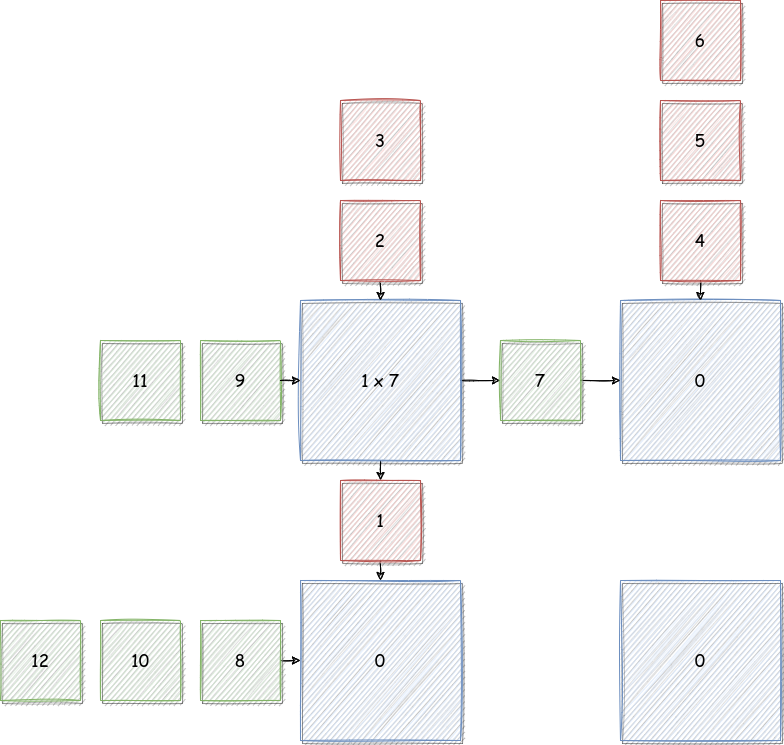
\includegraphics[width=0.6\linewidth]{img/矩阵乘原理.png}
    \caption{矩阵乘原理}
\end{figure} 


\subsection{Verilog实现}

在Verilog中,可以支持$8 * \text{num}$的Feature矩阵和$\text{num} * 8$的Weight矩阵相乘,实现最后的输出。

在这里,Feature矩阵是横向输入的,Weight矩阵是纵向输入的,由基本单元MAC映射结果矩阵的每个元素,进行计算。

\subsubsection{外部接口}

使用MAC作为基本单元,为了减少电路的旁路,MAC使用了大量的数据在MAC中进行串行传递

在计算过程中,会有如下数据的传递:

\begin{itemize}
\item
  矩阵大小参数num:整个计算单元仅有唯一的输入,输入到位于\((0, 0)\)位置的MAC,接下来,位于第一列的MAC进行从上到下的传递,每一行进行从左到右的传递
\item
  w矩阵的数据:为纵向传递,第一行的MAC接收外部输入
\item
  f矩阵的数据:为横向传递,第一列的MAC接收外部输入
\item
  结果输出:纵向传递,先传输的为行号高的数据
\end{itemize}

\subsubsection{计算单元MAC}

MAC的作用有两个:

\begin{enumerate}
\item
  计算乘加操作,当w和f数据均为valid时,进行乘,并累加到自身的寄存器上,累加次数为num,实现了矩阵乘法操作
\item
  数据传递:满足需要传递数据时,自身数据已经先行传递出去了,故不会造成数据冲突
\end{enumerate}

\section{实验实现}

\subsection{问题1}

问题在于乘法的符号扩展问题:如果\texttt{f\_data}的符号扩展类型为无符号,则乘法结果也是无符号的。

第一组矩阵乘的Feature矩阵均为正数,故不会造成影响;而第二组矩阵乘的Feature中元素有负数,故乘法过程中会造成错误,负数按照无符号类型进行扩展,造成了结果的错误。

故需要进行如下的修改:

\begin{lstlisting}
- assign f_data_extend = $signed(8'b0, f_data});
+ assign f_data_extend = $signed({{8{f_data[7]}}, f_data});
\end{lstlisting}

修改后,可以得到正确的波形:

\begin{figure}[htbp]
    \centering
    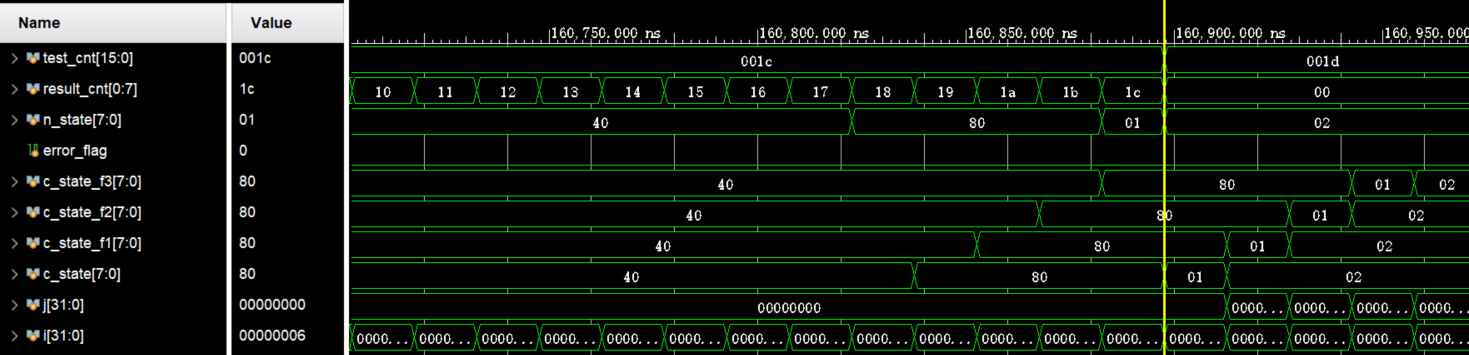
\includegraphics[width=0.8\linewidth]{img/wave.png}
    \caption{wave}
\end{figure} 

\subsection{问题2}

\subsubsection{MAC的接口与功能定义}

MAC的接口定义为:

\begin{longtable}[]{@{}l|l|l|l@{}}
\toprule\noalign{}
信号名 & 位宽 & 方向 & 含义 \\
\midrule\noalign{}
\endhead
\bottomrule\noalign{}
\endlastfoot
num\_valid & 1 & I & 握手信号:矩阵参数num是否有效 \\
num & 32 & I & 矩阵参数num \\
num\_valid\_r & 1 & O & 上一拍的握手信号:用于传递给其他MAC \\
num\_r & 32 & O & 上一拍的矩阵参数num:用于传递给其他MAC \\
w\_valid & 1 & I & 握手信号:传入的w\_data是否有效 \\
w\_data & 8 & I & weight矩阵数据 \\
w\_valid\_r & 1 & O & 上一拍的握手信号:用于传递给其他MAC \\
w\_data\_r & 8 & O & 上一拍的weight矩阵数据:用于传递给其他MAC \\
f\_valid & 1 & I & 握手信号:传入的f\_data是否有效 \\
f\_data & 8 & I & feature矩阵数据 \\
f\_valid\_r & 1 & O & 上一拍的握手信号:用于传递给其他MAC \\
f\_data\_r & 8 & O & 上一拍的feature矩阵数据:用于传递给其他MAC \\
valid\_l & 1 & I & 握手信号:下一个(下方)MAC的数据是否有效 \\
data\_l & 8 & I & 下一个(下方)MAC的数据 \\
valid\_o & 1 & O & 当前MAC运算结果是否有效 \\
data\_o & 8 & O & MAC的输出数据 \\
\end{longtable}

MAC的数据流向是确定的:

\begin{itemize}
\item
  矩阵大小参数num:整个计算单元仅有唯一的输入,输入到位于\((0, 0)\)位置的MAC,接下来,位于第一列的MAC进行从上到下的传递,每一行进行从左到右的传递
\item
  w矩阵的数据:为纵向传递,第一行的MAC接收外部输入
\item
  f矩阵的数据:为横向传递,第一列的MAC接收外部输入
\item
  结果输出:纵向传递,先传输的为行号高的数据
\end{itemize}

故输出数据的选择其实是确定的:当下方MAC数据有效时,自身的数据一定已经传输出去了,故可以进行选择下方传入的数据

至于为什么不再设置一个传输数据输出的端口,合理的猜测是为了节省不必要的电路资源消耗

\subsubsection{Multipy的接口和定义}

事实上Multipy过于糟糕的写法造成了极低的可读性,进行重构后可以明白其清晰的逻辑:

\begin{enumerate}
\item
  计算的过程是通过数据传递实现的,当数据进行输入时,也就同时开始计算,传输完成时数据也就完成了计算
\item
  当数据完成计算后,开始进行数据的输出
\end{enumerate}

Multipy的接口定义:

\begin{longtable}[]{@{}l|l|l|l@{}}
\toprule\noalign{}
信号名 & 位宽 & 方向 & 含义 \\
\midrule\noalign{}
\endhead
\bottomrule\noalign{}
\endlastfoot
clk & 1 & I & 时钟信号 \\
rst & 1 & I & 异步复位信号,高电平有效 \\
fvalid & 1 & I & 握手信号:输入的feature矩阵数据是否有效 \\
fdata & 8 & I & 输入的feature矩阵数据 \\
wvalid & 1 & I & 握手信号:输入的weight矩阵数据是否有效 \\
wdata & 8 & I & 输入的weight矩阵数据 \\
num\_valid\_ori & 1 & I & 握手信号:输入的num数据是否有效 \\
num\_ori & 32 & I & 矩阵参数num \\
valid\_o & 1 & O & 握手信号:矩阵输出数据是否有效 \\
data\_o & 32 & O & 矩阵输出数据 \\
\end{longtable}

比如num的传递逻辑,为第一列进行从上至下的传递,第一列的元素再从左向右进行传递,故代码为:

\begin{lstlisting}
generate
    for(i = 0; i < 8; i = i + 1) begin
        for(j = 0; j < 8; j = j + 1) begin
            if(j == 0) begin
                // (0, 0)MAC为输入
                if(i == 0) begin
                    assign num_valid[8 * i + j] = num_valid_ori;
                    assign num[8 * i + j]       = num_ori;
                end
                // 每行第一个接受上方传入
                else begin
                    assign num_valid[8 * i + j] = num_valid_r[8 * (i - 1) + j];
                    assign num[8 * i + j]       = num_r[8 * (i - 1) + j];
                end
            end
            // 一般的MAC由左边的单元进行传递
            else begin
                assign num_valid[8 * i + j]     = num_valid_r[8 * i + j - 1];
                assign num[8 * i + j]           = num_r[8 * i + j - 1];
            end
        end
    end
endgenerate
\end{lstlisting}

类似的,Weight矩阵、Feature矩阵、结果输出矩阵的传递思路都类似,只是传递方向有横向和纵向的区别,就不再赘述。

\section{实验结果与分析}

实现了矩阵乘法。

核心在于MAC中数据流交互,实现了乘加操作。

同时,利用矩阵参数num作为计数器,表示一共要进行多少次计算。

\section{实验总结}

实现了良好的矩阵乘效果。

\end{document}